\section{Reaktans til Impedans}
Reaktans:

Ved et LCR-kredsløb, så er der ikke kun tale om modstanden fra resistoren, men hvilken modstand kapacitoren og induktoren har. Den samlede modstand for kredsløbet kan beskrives igennem kompleks impedans, som er den samlede modstand for resistoren, kapacitoren og induktoren på kompleks form. Impedansen er essentiel til beskrivelse af den faseforskydelse, der kan opstå mellem spændingen og strømstyrken i LCR-kredsløbet.

For at forstå modstanden for en kapacitor og induktor, så skal begrebet reaktans bringes på banen. Ved elektriske felter er der tale om kapacitiv reaktans, som er gældende for kapacitorer, mens der for magnetiske felter er tale om induktiv reaktans, som er gældende for induktorer. Reaktansen for henholdsvis kapacitoren og induktoren er angivet, som deres modstand og optræder efter sammenhængen mellem strømstyrken og spændingen over kapacitoren og induktoren. Da de to komponenter ikke optræder ens i kredsløbet, er beregningerne for reaktansen forskellig.

\begin{equation}
Kapacitiv reaktans: X_C = - \frac{1}{j \omega C}
\label{eq:kapacitivreaktans}
\end{equation}
\begin{equation}
Induktiv reaktans: X_L = j \omega L
\label{eq:induktivreaktans}
\end{equation}

I formel \ref{eq:kapacitivreaktans} og \ref{eq:induktivreaktans} indgår der to konstanter $C$ og $L$. C er en konstant for kapacitoren angivet som kapacitansen, mens $L$ er en konstant for induktoren angivet som induktansen. Omega beskrives som $\omega = 2 \pi f$, hvor $2 \pi$ svarer til én svingning, mens $f$ er frekvensen. $j$ angiver, at reaktansen er beskrevet som et kompleks tal.

Komplekse tal bliver benyttet for bedre, at kunne knytte spænding og strømstyrke sammen, så det kan afbilledes i forbindelse med den fastforskydelse, der kan forekomme. Dette forhold mellem spænding og strømstyrke kan udledes gennem omskrivning af sinus og cosinus, men for nemhedens skyld benyttes komplekse tal for at simplificere formlerne. Formlerne for reaktansen kan derved skrives om til:

\begin{equation} 
Kapacitiv reaktans: X_C = - \frac{1}{j 2 \pi f C}
\end{equation}
\begin{equation}
Induktiv reaktans: X_L = j 2 \pi f L
\end{equation}
%Kilde: Reactance of capacitors and inductors

En perfekt kapasitor uden modstand ville forskyde bølgefunktionen for strømstyrken med $\frac{\pi}{2}$ frem for bølgefunktionen for spænding., hvilket svarer til en kvart svingning (1/4 frekvens). Modsat ville den perfekte induktor uden modstand sænke bølgefunktionen for strømstyrken med $\frac{\pi}{2}$ i forhold til bølgefunktionen for spænding.

Billeder af forskudte bølger (kapacitiv og induktiv reaktans)
\begin{figure}[H]
\centering
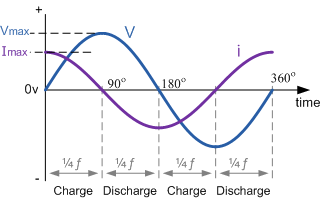
\includegraphics[scale=1]{Vildledning/Schematics/Kapacitiv_reaktans}
\caption{Kapacitiv reaktans}
\label{kreaktans}
\end{figure}
%Kilde: Capacitance in AC Circuit and Capacitive Reactance

\begin{figure}[H]
\centering
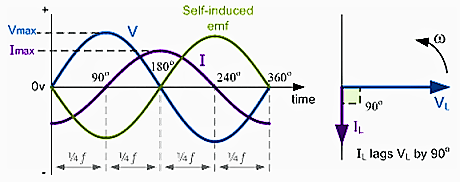
\includegraphics[scale=0.8]{Vildledning/Schematics/Induktiv_reaktans}
\caption{Induktiv reaktans}
\label{ireaktans}
\end{figure}
%Kilde: Inductive Reactance - Reactance of an Inductor

Da den komplekse impedans var LCR-kredsløbets samlede modstand, så kan det beregnes ved:
\begin{equation}
Z = R + j 2 \pi f L - \frac{1}{j 2 \pi f C}
\end{equation}
%Kilde: Complex Impedance
\newpage